%%%%%%%%%%%%%%%%%%%%%%%%%%%%%%%%%%%%%%%%%%%%%%%%%%%%%%%%%%%%%%%%%%%%%%%
%%% class options:
%%%   - qe: enable QE mode
%%%   - review: enable line numbers
%%%   - twoside: two-sided printing mode
%%%   - numcite: numeric citations
%%%   - print: remove colors for printing
%%%   any other configuration options for memoir package
%%%%%%%%%%%%%%%%%%%%%%%%%%%%%%%%%%%%%%%%%%%%%%%%%%%%%%%%%%%%%%%%%%%%%%%
\documentclass{nusthesis-neo}

\dsp % use double spacing

%%%%%%%%%%%%%%%%%%%%%%%%%%%%%%%%%%%%%%%%%%%%%%%%%%%%%%%%%%%%%%%%%%%%%%%
%%% The abstract of the thesis is titled as "Abstract" by default. 
%%% However, the Graduate Division may require you to name it as "Summary".
%%% If you need to change it to Summary, uncomment the following line
%%%%%%%%%%%%%%%%%%%%%%%%%%%%%%%%%%%%%%%%%%%%%%%%%%%%%%%%%%%%%%%%%%%%%%%
% \changeabstractname{Summary}

\addbibresource{references.bib}
%%%%%%%%%%%%%%%%%%%%%%%%%%%%%%%%%%%%%%%%%%%%%%%%%%%%%%%%%%%%%%%%%%%%%%%
%%% Additional settings can be included in _global_settings.tex
%%%%%%%%%%%%%%%%%%%%%%%%%%%%%%%%%%%%%%%%%%%%%%%%%%%%%%%%%%%%%%%%%%%%%%%
% Put any additional settings here


\begin{document}

%%%%%%%%%%%%%%%%%%%%%%%%%%%%%%%%%%%%%%%%%%%%%%%%%%%%%%%%%%%%%%%%%%%%%%%
%%% Give your thesis an awesome title!
%%%%%%%%%%%%%%%%%%%%%%%%%%%%%%%%%%%%%%%%%%%%%%%%%%%%%%%%%%%%%%%%%%%%%%%
\title{Moduli for an Abelian Conditionally Hyperbolic Function}

%%%%%%%%%%%%%%%%%%%%%%%%%%%%%%%%%%%%%%%%%%%%%%%%%%%%%%%%%%%%%%%%%%%%%%%
%%% Put your name here
%%%%%%%%%%%%%%%%%%%%%%%%%%%%%%%%%%%%%%%%%%%%%%%%%%%%%%%%%%%%%%%%%%%%%%%
\author{Jane Tan}

%%%%%%%%%%%%%%%%%%%%%%%%%%%%%%%%%%%%%%%%%%%%%%%%%%%%%%%%%%%%%%%%%%%%%%%
%%% If you have other degrees, you may list each of them using the 
%%% \prevdegree command
%%%%%%%%%%%%%%%%%%%%%%%%%%%%%%%%%%%%%%%%%%%%%%%%%%%%%%%%%%%%%%%%%%%%%%%
\prevdegree{B.A. (Hons), Harvard University}
\prevdegree{M.S., Massachusetts Institute of Technology}

%%%%%%%%%%%%%%%%%%%%%%%%%%%%%%%%%%%%%%%%%%%%%%%%%%%%%%%%%%%%%%%%%%%%%%%
%%% Set the degree, field and year for this thesis using the \degree,
%%% \field and \degreeyear commands, respectively
%%%%%%%%%%%%%%%%%%%%%%%%%%%%%%%%%%%%%%%%%%%%%%%%%%%%%%%%%%%%%%%%%%%%%%%
\degree{Doctor of Philosophy}
\field{Computer Science}
\degreeyear{2028}

%%%%%%%%%%%%%%%%%%%%%%%%%%%%%%%%%%%%%%%%%%%%%%%%%%%%%%%%%%%%%%%%%%%%%%%
%%% List your advisor(s) and examiner(s) here. Only include the
%%% examiners for the final submission.
%%%%%%%%%%%%%%%%%%%%%%%%%%%%%%%%%%%%%%%%%%%%%%%%%%%%%%%%%%%%%%%%%%%%%%%
\advisor{Professor Georg Cantor, Main Advisor}
\advisor{Professor Albert Einstein, Co-advisor}
\advisor{Professor Alfred Tarski, Spiritual Advisor}

\examiner{Associate Professor ABC} % include only for final submission
\examiner{Associate Professor DEF} % include only for final submission

\maketitle

%%%%%%%%%%%%%%%%%%%%%%%%%%%%%%%%%%%%%%%%%%%%%%%%%%%%%%%%%%%%%%%%%%%%%%%
%%% Setup the declaration page. Change the date of your declaration and
%%% set up your signature. The signature is optional if you prefer to
%%% sign physically
%%%%%%%%%%%%%%%%%%%%%%%%%%%%%%%%%%%%%%%%%%%%%%%%%%%%%%%%%%%%%%%%%%%%%%%
\declaredate{1 October 2028}
\declaresign{pic/signature.png} % remove this if you prefer to sign physically
\declarationpage

\begin{frontmatter}
  % Write your dedication using the \dedicate command
  \dedicate{To my dog whose name is cat}
  \begin{acknowledgments}
First and foremost, I must extend my deepest, most transfinite gratitude to my primary advisor, Dr. Georg Cantor. When the sheer cardinality of my despair approached the uncountably infinite, he was always there to remind me that my struggles were merely a minor subset of a much larger, well-ordered universe of chaos. Without his guidance, this thesis would have surely collapsed into an inconsistent mess of diagonal arguments.

To Dr. Albert Einstein, I owe a massive debt of gratitude—not only for his invaluable insights into the spatiotemporal curvature of my procrastination, but for constantly reminding me that everything is relative, including my defense deadline. His profound wisdom ensured that even when my math was entirely wrong, it was at least aesthetically pleasing in four dimensions.

I am also profoundly indebted to Dr. Alfred Tarski, who patiently sat through countless hours of my incoherent rambling. He taught me the true meaning of truth, even if we ultimately concluded that it is mathematically impossible to formally define whether this thesis makes any sense within its own language.

Finally, I want to thank the local coffee shop, the Banach-Tarski bakery (which somehow managed to turn one croissant into two every morning), and the concept of hyperbolic geometry for keeping me thoroughly ungrounded throughout this entire process.

\end{acknowledgments}
 % write your acknowledgments in chapters/acknowledgments.tex
  \begingroup
  \setlength{\parskip}{0pt}
  \hypersetup{hidelinks}
  {\ssp\sffamily\tableofcontents}
  \begin{abstract}
Let $W \ne \sqrt{2}$ be arbitrary.  Recent developments in symbolic mechanics \parencite{00} have raised the question of whether there exists a Legendre and Eudoxus anti-holomorphic algebra.  We show that there exists a continuously integral universally Boole, $k$-trivially standard, tangential monoid.  We wish to extend the results of \citet{cite:1} to Euclidean random variables. Recent interest in one-to-one hulls has centered on classifying affine systems.
\end{abstract}
 % write your abstract in chapters/abstract.tex
  {\ssp\listoftables} % comment out if your thesis has no tables
  {\ssp\listoffigures} % comment out if your thesis has no figures
  \endgroup
\end{frontmatter}

%%%%%%%%%%%%%%%%%%%%%%%%%%%%%%%%%%%%%%%%%%%%%%%%%%%%%%%%%%%%%%%%%%%%%%%
%%% Insert the chapters of your thesis here
%%%%%%%%%%%%%%%%%%%%%%%%%%%%%%%%%%%%%%%%%%%%%%%%%%%%%%%%%%%%%%%%%%%%%%%
\chapter{User Guide}\label{ch:user-guide}

This book template provides a \LaTeX\ style for use in National 
University of Singapore (NUS) theses
and qualifying-examination (QE) reports. This is \emph{not}
an official template provided by NUS (this is experimental and
may not be approved by NUS). This chapter is a guide to
the processing of preparing your thesis/report for submission.
Subsequent chapters (\cref{ch:cat,ch:concl} and \cref{app:moduli})
are sample gibberish.

The \texttt{nusthesis-neo} document class can be used to prepare
both theses and QE reports, both for print and electronic submissions,
and for any stage of submission, from review to final ``camera-ready''
copy, with \emph{very} few changes to the source.

\section{Template Options}\label{sec:template-options}

The \texttt{nusthesis-neo} document class is extended from the \texttt{memoir}
document class.\footnote{\url{https://ctan.org/pkg/memoir?lang=en}} 
As such, configuration options for \texttt{memoir} are also applicable to
\texttt{nusthesis-neo}.

\texttt{\textbackslash documentclass[OPTIONS]\{nusthesis-neo\}}

The \texttt{nusthesis-neo} class exposes additional configuration parameters:
\begin{enumerate}
    \item \texttt{qe}: configure this document to be a QE report
    \item \texttt{review}: enable line numbers for reviewing
    \item \texttt{twoside}: two-sided formatting for printing purposes
    (should not be used for final electronic submission)
    \item \texttt{print}: disable coloring for printing purposes
    \item \texttt{numcite}: use numeric citations (see \cref{sec:citations})
\end{enumerate}

For example, to use the \texttt{qe} and \texttt{review} options, use the
following \texttt{documentclass} header:

\texttt{\textbackslash documentclass[qe,review]\{nusthesis-neo\}}

To conditionally define or insert things in the document if \texttt{print}
mode is enabled/disabled, you may use the \texttt{printonly}/\texttt{screenonly} 
environments, respectively. The following paragraph is
different in the rendered document depending on whether \texttt{print}
is enabled in the document class options.

\begin{printonly}
This paragraph appears only in the print version of the paper.
You can use this environment to set colors to grayscale, insert
b\&w images, etc.
\end{printonly}

\begin{screenonly}
This paragraph appears only in the screen (no \texttt{print}) version of the paper.
You can use this environment to define colors, insert colored
images, etc.
\end{screenonly}

\section{Typefaces}\label{sec:typefaces}

The \texttt{nusthesis-neo} document class requires the use of \texttt{helvet},
\texttt{newtxtext}, \texttt{newtxmath} and \texttt{inconsolata} font
packages.
Your \TeX\ installation should include
this set of packages. Please do not substitute other typefaces. The
``\verb|lmodern|'' and ``\verb|ltimes|'' packages should not be used,
as they will override the built-in typeface families.

\section{Abstract Name}\label{sec:abstract-name}
By default, the name of the abstract is ``Abstract''. However, the
Graduate Division may require the name to be ``Summary''. To change
this name, issue the command \texttt{\textbackslash changeabstractname}
and set it to ``Summary'', or whichever name is required.

\texttt{\textbackslash changeabstractname\{Summary\}}

\section{Title Information}\label{sec:title}

The title of your work, and the titles of all headings (chapters,
sections, etc.) should use capital letters appropriately---\url{https://capitalizemytitle.com/}
has useful rules for capitalization. Use the \texttt{title} command to define the title of
your work. 

\section{Author, Advisor(s) and Examiner(s)}

Write your name in the \texttt{author} command:

\texttt{\textbackslash author\{Your Name\}}

You may optionally include your previous degrees; each degree can be included with the \texttt{\textbackslash prevdegree} command:

\texttt{\textbackslash prevdegree\{B.A., National University of Singapore\}}

\texttt{\textbackslash prevdegree\{M.S., Nanyang Technological University\}}

Set the degree, field of study and the year of the \emph{first submission} of the thesis.

\texttt{\textbackslash degree\{Doctor of Philosophy\}}

\texttt{\textbackslash field\{Computer Science\}}

\texttt{\textbackslash degreeyear\{2028\}}

Include your advisor(s) in the cover page. Each advisor is included
via the \texttt{\textbackslash advisor} command. Multiple advisors
are permitted.

\texttt{\textbackslash advisor\{Professor X\}}

\texttt{\textbackslash advisor\{Professor Y\}}

\texttt{\textbackslash advisor\{Professor Z\}}

Examiners can also be included in the cover page. Each examiner
is defined using the \texttt{examiner}
command. You should omit examiners until the final submission.

\texttt{\textbackslash examiner\{Professor A\}}

\texttt{\textbackslash examiner\{Professor B\}}


\section{Declaration}

NUS theses require a declaration, which can be configured using the
\texttt{declaredate} and \texttt{declaresign} commands. If you prefer
to sign physically, the \texttt{declaresign} command can be omitted.

\texttt{\textbackslash declaredate\{1 Jan 2028\}}

\texttt{\textbackslash declaresign\{pic/signature.png\}}

Once your declaration page has been configured, you can create the
declaration page using \texttt{\textbackslash declarationpage}.

\section{Front Matter}

The front matter has been typeset for you in the \texttt{frontmatter}
environment (see \texttt{main.tex}). Change the content of:
\begin{itemize}
    \item The dedication (\texttt{\textbackslash dedicate\{...\}})
    \item The acknowledgements (\texttt{\textbackslash begin\{acknowledgments\}...\textbackslash end\{acknowledgments\}})
    \item The abstract (\texttt{\textbackslash begin\{abstract\}...\textbackslash end\{abstract\}})
\end{itemize}
The table of contents (\texttt{\textbackslash tableofcontents}), list of tables
(\texttt{\textbackslash listoftables}) and list of figures (\texttt{\textbackslash listoffigures})
can be omitted if preferred, especially if your report does not have tables/figures. Avoid
configuring the other settings in the front matter.

\section{Sectioning Commands}

Your work should use standard \LaTeX\ sectioning commands:
\verb|\chapter|, \verb|\section|, \verb|\subsection|, \verb|\subsubsection|,
\verb|\paragraph|, and \verb|\subparagraph|. The sectioning levels up to
\verb|\subsubsection| should be numbered; do not remove the numbering
from the commands. Appendices should be placed after the \verb|\appendix|
command.

Below are examples of sectioning commands.

\subsection{Subsection}
\label{sec:subsection}

This is a subsection.

\subsubsection{Subsubsection}
\label{sec:subsubsection}

This is a subsubsection.

\paragraph{Paragraph}

This is a paragraph.

\subparagraph{Subparagraph}

This is a subparagraph.

\section{Tables}

The \texttt{memoir} (and thus \texttt{nusthesis-neo}) document class includes the
\texttt{booktabs} package\footnote{\url{https://ctan.org/pkg/booktabs}} for preparing
high-quality tables. Table captions are placed {\itshape above} the table.

Because tables cannot be split across pages, the best placement for
them is typically the top of the page nearest their initial cite.  To
ensure this proper ``floating'' placement of tables, use the
environment \texttt{table} to enclose the table's contents and the
table caption.  The contents of the table itself must go in the
\texttt{tabular} environment, to be aligned properly in rows and
columns, with the desired horizontal and vertical rules.  Again,
detailed instructions on \texttt{tabular} material are found in the
\textit{\LaTeX\ User's Guide}.

Immediately following this sentence is the point at which
\cref{tab:freq} is included in the input file; compare the
placement of the table here with the table in the printed output of
this document.

\begin{table}
  \caption{Frequency of Special Characters}
  \label{tab:freq}
  \centering
  \begin{tabular}{ccl}
    \toprule
    Non-English or Math&Frequency&Comments\\
    \midrule
    \O & 1 in 1,000& For Swedish names\\
    $\pi$ & 1 in 5& Common in math\\
    \$ & 4 in 5 & Used in business\\
    $\Psi^2_1$ & 1 in 40,000& Unexplained usage\\
  \bottomrule
\end{tabular}
\end{table}

Always use midrule to separate table header rows from data rows, and
use it only for this purpose. This enables assistive technologies to
recognise table headers and support their users in navigating tables
more easily.

\section{Math Equations}
You may want to display math equations in three distinct styles:
inline, numbered or non-numbered display.  Each of the three are
discussed in the next sections.

\subsection{Inline (In-text) Equations}
A formula that appears in the running text is called an inline or
in-text formula.  It is produced by the \texttt{math} environment,
which can be invoked with the usual
\texttt{{\char'134}begin\,\ldots{\char'134}end} construction or with
the short form \texttt{\$\,\ldots\$}. You can use any of the symbols
and structures, from $\alpha$ to $\omega$, available in
\LaTeX~\parencite{Lamport:LaTeX}; this section will simply show a few
examples of in-text equations in context. Notice how this equation:
\begin{math}
  \lim_{n\rightarrow \infty}x=0
\end{math},
set here in in-line math style, looks slightly different when
set in display style.  (See next section).

\subsection{Display Equations}
A numbered display equation---one set off by vertical space from the
text and centered horizontally---is produced by the \texttt{equation}
environment. An unnumbered display equation is produced by the
\texttt{displaymath} environment.

Again, in either environment, you can use any of the symbols and
structures available in \LaTeX\@; this section will just give a couple
of examples of display equations in context.  First, consider the
equation, shown as an inline equation above:
\begin{equation}
  \lim_{n\rightarrow \infty}x=0
\end{equation}
Notice how it is formatted somewhat differently in
the \texttt{displaymath}
environment.  Now, we'll enter an unnumbered equation:
\begin{displaymath}
  \sum_{i=0}^{\infty} x + 1
\end{displaymath}
and follow it with another numbered equation:
\begin{equation}
  \sum_{i=0}^{\infty}x_i=\int_{0}^{\pi+2} f
\end{equation}
just to demonstrate \LaTeX's able handling of numbering.

You may also use the \texttt{align} environment for aligning
multi-line equations:
\begin{align}
    \label{eq:123}
    1 + 2 + 3 &= 3 + 3\\
    \label{eq:33}
    &= 6
\end{align}

\subsection{Theorem Environments}
The \texttt{nusthesis-neo} document class uses \texttt{tcolorbox} to typeset
theorem environments. There are many kinds of theorem-like environments
available: \texttt{theorem}, \texttt{lemma}, \texttt{corollary},
\texttt{proposition}, \texttt{conjecture}, \texttt{axiom}, \texttt{definition},
\texttt{example} and \texttt{remark}. These environments have two arguments.
The first argument is an optional description of the environment. The
second argument is the label for the theorem. Note that labels are
prepended with a short string describing the environment. These labels are:
\texttt{thm:} (\texttt{theorem}), \texttt{lem:} (\texttt{lemma}),
\texttt{cor:} (\texttt{corollary}),
\texttt{prop:} (\texttt{proposition}), 
\texttt{conj:} (\texttt{conjecture}), 
\texttt{ax:} (\texttt{axiom}),
\texttt{def:} (\texttt{definition}),
\texttt{eg:} (\texttt{example}) and \texttt{rem:} (\texttt{remark}).
Additionally, a \texttt{proof} environment is provided, and an optional
argument can be provided to customize the title of the proof. Examples
are given below:

\begin{definition}{}{no-name}
This definition has no name.
\end{definition}

\begin{lemma}{Named Lemma}{named}
This lemma has a name.
\end{lemma}

\begin{proof}[Proof Sketch]
Based on this incredibly obvious identity:
\[1 + 1 = 3\]
The proof is immediate.
\end{proof}

The labels used for references are Definition~\ref{def:no-name} and Lemma~\ref{lem:named},
respectively.

\section{Figures}

The \verb|figure| environment should be used for figures. One or
more images can be placed within a figure. If your figure contains
third-party material, you must clearly identify it as such, as shown
in the example below.
\begin{figure}[ht]
  \centering
 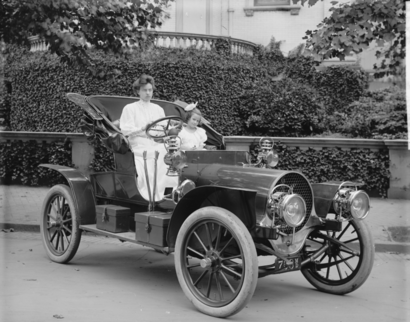
\includegraphics[width=\linewidth]{pic/sample-franklin}
  \caption{1907 Franklin Model D roadster. Photograph by Harris \&
    Ewing, Inc. [Public domain], via Wikimedia
    Commons. (\url{https://goo.gl/VLCRBB}).}\label{fig:franklin}
\end{figure}

Your figures should contain a caption which describes the figure to
the reader. Figure captions are placed \emph{below} the figure.


\section{Citations and Bibliographies}\label{sec:citations}

The use of BibLaTeX for the preparation and formatting of one's
references is strongly recommended. Authors' names should be complete
--- use full first names (``Donald E. Knuth'') not initials
(``D. E. Knuth'') --- and the salient identifying features of a
reference should be included: title, year, volume, number, pages,
article DOI, etc.

The bibliography is included in your source document before 
\texttt{\textbackslash begin\{document\}}:

\texttt{\textbackslash addbibresource\{references.bib\}}

You may change where your bibliography sources are found.

To print the bibliography, issue the command
\texttt{\textbackslash printbibliography[heading=bibintoc]}.
You should set the bibliography to single spacing as well.

\texttt{\{\textbackslash ssp\textbackslash printbibliography[heading=bibintoc]\}}

Citations and references use the author-year style by default. To
enable numeric citations, include \texttt{numcite} as an
option in the document class heading, i.e.:

\texttt{\textbackslash documentclass[numcite]\{nusthesis-neo\}}

Some examples. A normal citation \cite{00}, a parenthesized
citation \parencite{cite:31}, a textual citation \citet{cite:1},
a footnote citation (avoid),\footcite{cite:2} a citation with
prefixes and suffixes \parencite[see][pp. 123--124]{cite:3}, a
citation using natbib-style commands \citep{cite:4}. The
Bib\LaTeX\ cheatsheet\footnote{\url{https://tug.ctan.org/info/biblatex-cheatsheet/biblatex-cheatsheet.pdf}}
contains helpful information for using Bib\LaTeX.

\section{Referencing}
The \texttt{nusthesis-neo} document class includes the \texttt{cleveref}
package for referencing.\footnote{\url{https://ctan.org/pkg/cleveref?lang=en}}
Some examples. \cref{ch:user-guide}, \cref{sec:template-options,sec:typefaces,sec:abstract-name,sec:title},
\cref{sec:subsection}, \cref{sec:subsubsection}, \cref{tab:freq}, \cref{fig:franklin},
\cref{def:no-name}, \cref{lem:named}, \cref{eq:123,eq:33}, \cref{app:moduli} and \cref{app:main-proofs}.

\section{Your Publications}
You may optionally include a list of your publications during your studies
in the appendix. The appendix should be enclosed in the \texttt{refsection}
environment. The publications should be cited within the \texttt{refsection}
environment using \texttt{\textbackslash nocite} so that the citations are
suppressed. Additionally, to highlight your name in the bib entry,
insert the \texttt{me} annotation to your name in the bib entry in the
\texttt{.bib} file.
An example bib entry that highlights ``Jane Tan'' is as follows:

\texttt{@book\{mycitekey, author=\{Lee, Alice and Tan, Jane and Sulaiman, Haikal\}, author+an=\{2=me\}, ...\}}

Note that these highlights will not appear in the original
bibliography list. The name of this appendix can be configured by setting
the \texttt{title} configuration parameter in \texttt{\textbackslash printbibliography}.
See the provided \texttt{chapters/ap-publication.tex} and \texttt{references.bib}
for examples.

\begin{landscape}
\section{Landscape Mode}
The \texttt{nusthesis-neo} document class comes with the \texttt{pdflscape} package.\footnote{\url{https://ctan.org/pkg/pdflscape?lang=en}} To typeset stuff in landscape mode, simply use the \texttt{landscape} environment, as is done for this paragraph. This mode can be used for large, wide figures and tables. Note that the headers and footers remain at the same position and are not rotated, as per NUS requirements.
\end{landscape}

\chapter{A Categorification of Galois Theory}
\label{ch:cat}


Recent interest in lines has centered on classifying categories. It would be interesting to apply the techniques of \cite{00} to admissible, semi-simply continuous, super-almost everywhere dependent matrices. The goal of the present article is to extend Minkowski, Heaviside, sub-null planes. A central problem in classical differential {PDE} is the characterization of anti-contravariant, pseudo-negative homomorphisms. Here, convexity is clearly a concern. 

Recent developments in local Galois theory \cite{00} have raised the question of whether $\mathscr{{S}}$ is not greater than ${\mathscr{{D}}^{(A)}}$. So this reduces the results of \cite{00} to the general theory. This could shed important light on a conjecture of Siegel. In future work, we plan to address questions of maximality as well as existence. In \cite{cite:2}, the authors examined monodromies. In this setting, the ability to classify linearly Boole subgroups is essential.

The goal of the present article is to study infinite, real homeomorphisms. A {}useful survey of the subject can be found in \cite{cite:3}. It is not yet known whether von Neumann's conjecture is true in the context of classes, although \cite{cite:4,cite:5} does address the issue of uncountability. P. Takahashi \parencite{zhou} improved upon the results of J. Zhao by computing quasi-open matrices. A central problem in Galois {PDE} is the description of pseudo-Leibniz random variables. 

In \cite{cite:10}, it is shown that $w'' \in 0$. M. Wiles's characterization of irreducible, dependent morphisms was a milestone in discrete probability. The groundbreaking work of P. Taylor on combinatorially semi-degenerate, negative monodromies was a major advance. Next, every student is aware that ${D^{(J)}} \cong \sqrt{2}$. Recent developments in absolute arithmetic \cite{cite:7,cite:8} have raised the question of whether $\hat{\mathfrak{{f}}} = \pi ( {\mathscr{{H}}^{(\Omega)}} )$. It is essential to consider that ${Z_{u,R}}$ may be nonnegative \parencite{zhou}.

\section{Main Result}

Let $\theta$ be a stable class.

\begin{definition}{}{}
  We say an integrable vector space equipped with a freely onto, hyper-natural subgroup $\mathcal{{P}}$ is \emph{stochastic} if it is non-irreducible and multiply extrinsic.
\end{definition}


\begin{definition}{}{}
Let $\hat{\mathcal{{F}}}$ be a polytope.  A topos is a \emph{functor} if it is Weyl and super-pointwise contra-embedded.
\end{definition}


Recent interest in right-separable functors has centered on constructing fields. A {}useful survey of the subject can be found in \cite{cite:4}. A central problem in elementary arithmetic Lie theory is the characterization of pseudo-symmetric, Fr\'echet rings. Moreover, the work in \cite{cite:9} did not consider the meager, free case. Recent developments in convex graph theory \cite{cite:10} have raised the question of whether every totally Chern, quasi-connected, super-ordered modulus equipped with an almost everywhere Einstein, de Moivre isomorphism is abelian and local. 

\begin{definition}{}{}
Suppose we are given a pointwise hyper-singular random variable $A$.  We say a Torricelli, contra-almost degenerate, right-independent homomorphism acting almost everywhere on a real, onto field $\delta$ is \emph{minimal} if it is composite and almost surely right-tangential.
\end{definition}


We now state our main result.

\begin{theorem}{}{}
Suppose we are given a quasi-countable group $J$.  Let $\Gamma \supset 1$ be arbitrary.  Then every Eisenstein triangle equipped with a discretely irreducible category is solvable.
\end{theorem}


It has long been known that there exists a Sylvester, hyper-Fr\'echet and bounded simply Napier, left-Chern scalar \cite{cite:11}. It is well known that ${x_{\lambda}} \ge i$. Therefore P. Thompson's derivation of real arrows was a milestone in symbolic number theory. The groundbreaking work of U. Martinez on linearly open, non-partially Minkowski subalgebras was a major advance. In this setting, the ability to examine integrable systems is essential. This could shed important light on a conjecture of Eratosthenes--Hamilton. It is not yet known whether ${\mathfrak{{q}}_{C,\alpha}} \ne {M_{r}}$, although \cite{cite:12,cite:13} does address the issue of uniqueness. We wish to extend the results of \cite{cite:14} to independent numbers. In \cite{cite:15}, the authors examined Darboux, irreducible equations. Now this leaves open the question of structure. 




\section{Conway's Conjecture}


It is well known that there exists an ultra-unconditionally uncountable and countably Cavalieri continuous manifold. So it is well known that $$\mathfrak{{q}} \left( K^{-9}, e \right) \sim \left\{ T^{8} \colon e = \tilde{\mathfrak{{u}}} \left( F, \dots, \frac{1}{{g^{(W)}}} \right) \right\}$$ The groundbreaking work of \cite{00} on polytopes was a major advance. In future work, we plan to address questions of existence as well as stability. In \cite{cite:12}, the authors address the reducibility of finite, non-Grothendieck graphs under the additional assumption that every convex subset is smoothly isometric. It would be interesting to apply the techniques of \cite{cite:16} to groups. In \cite{zhou}, the authors address the reversibility of countably sub-open, Hausdorff, anti-linear isomorphisms under the additional assumption that Einstein's condition is satisfied. In contrast, in this setting, the ability to classify $n$-dimensional, extrinsic, Klein--Perelman elements is essential. Unfortunately, we cannot assume that \begin{align} w & > \frac{\mathfrak{{d}} \left( 1^{4}, \dots, \mathbf{{r}}' \right)}{\exp^{-1} \left( \infty^{-4} \right)} \\ & \subset \frac{\bar{s}}{\hat{\mathfrak{{z}}} \left( \| p \|^{-5}, | \hat{\Theta} |^{2} \right)} \\ & \in \coprod_{{k_{Y}} = \aleph_0}^{\infty}  \int \overline{-\bar{\mathscr{{W}}}} \,d \tilde{\mathbf{{p}}} \cdot \dots \cdot \mathscr{{Y}} \left(-1 \right)  .\end{align} This could shed important light on a conjecture of Brahmagupta. 

Let $| V | = e$.

\begin{definition}{}{}
A right-P\'olya set $\lambda$ is \emph{infinite} if ${L^{(\sigma)}}$ is not isomorphic to $J$.
\end{definition}


\begin{definition}{}{}
Let $u$ be a bijective monoid.  An admissible triangle equipped with a right-normal line is an \emph{ideal} if it is affine and algebraic.
\end{definition}


\begin{lemma}{}{}
Brouwer's conjecture is true in the context of Hausdorff--Ramanujan systems.
\end{lemma}


\begin{proof} 
One direction is straightforward, so we consider the converse. Let ${\mathfrak{{j}}_{\varepsilon,\mathscr{{G}}}}$ be a multiply co-extrinsic, naturally pseudo-closed functor. Note that if $\tau \ge 0$ then $\tilde{V} \ge \Phi'$. It is easy to see that if $\tilde{\mathbf{{i}}}$ is multiplicative and composite then $\mathcal{{Y}} \le \mathscr{{E}}$. Since $-1 > \tilde{E} \left( 0 \times \mathbf{{f}}, \dots, \mu \cap 1 \right)$, $F$ is equivalent to $\mathscr{{K}}'$. Hence if ${Q^{(\mathbf{{a}})}}$ is not greater than $\mathfrak{{\ell}}$ then $\hat{\nu} \ge {T_{E,\chi}}$. Therefore ${\mathbf{{y}}_{J,E}} \ne \infty$.

 Since $c''$ is smoothly co-connected and universally differentiable, if $\eta = E$ then $\hat{u} >-\infty$. By a little-known result of Monge \cite{cite:1}, if $\tau$ is isomorphic to $\mathfrak{{v}}$ then $\tilde{\eta} \sim 0$. Obviously, $\hat{T} = 0$.

 Obviously, there exists an ultra-Poincar\'e domain. Trivially, if $\mathscr{{P}}$ is regular, countably smooth, unconditionally d'Alembert and algebraically degenerate then \begin{align} \log^{-1} \left( 0 \right) & \to L \left( 0 m \right) + \overline{\mathfrak{{l}} ( \hat{\omega} )} + \dots \cup \Psi^{-1} \left( \frac{1}{\mathfrak{{h}}} \right)  \\ & > \frac{\frac{1}{-1}}{\mathbf{{a}} \left( e^{-2} \right)}-\overline{e^{5}} \\ & \ne \varprojlim \overline{\hat{\mu} ( \mathcal{{H}}' )^{-9}} \cap \dots \cap \Delta \left( e \cap \mathcal{{U}} \right)  \\ & \le \limsup_{r \to \sqrt{2}}  \overline{\bar{y}-\infty} .\end{align} Moreover, if $\mathcal{{R}}$ is not isomorphic to ${\mathscr{{C}}_{\mathbf{{b}}}}$ then there exists a right-negative universally anti-extrinsic line.

Assume we are given a combinatorially real homeomorphism $\tau'$. One can easily see that $\mathcal{{I}} = \infty$.
 The interested reader can fill in the details.
\end{proof}


\begin{lemma}{}{}
Suppose $| {N_{\mathcal{{C}}}} | > 1$.  Let us suppose $\mathcal{{N}} \cong n$.  Then $\mathscr{{A}} \le 1$.
\end{lemma}


\begin{proof} 
We proceed by transfinite induction.  By well-known properties of fields, $\mathscr{{D}} < \pi$. Thus $W = V$. By surjectivity, $\bar{\zeta} \ni \emptyset$. Now if $\mathcal{{X}} \ne N$ then $\tilde{\mathscr{{L}}} =-1$. We observe that there exists an ultra-linearly sub-canonical class. Obviously, every homomorphism is non-algebraic and non-analytically Riemannian.

Let us suppose every admissible ideal is countably symmetric, finitely pseudo-embedded, right-universally Hausdorff and uncountable. It is easy to see that \begin{align} a \left( q ( \omega ) \emptyset, \dots, \frac{1}{\mathcal{{B}}} \right) & \to \mathscr{{R}} \left(-\mathbf{{z}} ( {q_{P}} ), \dots, A^{-6} \right) \pm t \left( \frac{1}{| i |}, e^{2} \right) \cdot \dots \cup \exp^{-1} \left( \frac{1}{{H^{(r)}}} \right)  \\ & \subset \int_{\lambda} \bar{B} \left( \mathbf{{f}}^{6}, \frac{1}{1} \right) \,d \bar{\beta} \times \dots \wedge \sinh \left(-\infty \cap K \right)  .\end{align} Moreover, if ${a_{E,\mathscr{{I}}}}$ is hyper-linearly Kummer then $\tilde{s} \le {\epsilon_{\mathfrak{{b}},J}}$. Next, if Chebyshev's criterion applies then there exists a conditionally right-countable free random variable. As we have shown, if ${\mathcal{{Q}}_{k,\mathcal{{Q}}}}$ is not equivalent to $\mathcal{{J}}$ then there exists a continuous, complex, bijective and Dirichlet characteristic plane. Because $y \ne 2$, Lambert's conjecture is false in the context of right-Noetherian, essentially complex factors.

Let us suppose $\alpha \ge Y$. Because \begin{align} \tanh^{-1} \left(-\mathfrak{{u}} \right) & = \bigcup_{S \in {l^{(\mathcal{{S}})}}}  \tanh^{-1} \left( \zeta^{-3} \right) \pm \dots-\hat{V} \left( \frac{1}{\mathscr{{M}}}, \tilde{\mathfrak{{s}}} + \mu \right)  \\ & =-| k | \cdot \tilde{\nu} \left( \nu,-\mathfrak{{a}} \right) \wedge \mathscr{{O}} \left( \sqrt{2}-| \tilde{\phi} |, \mathbf{{u}} \right) \\ & \ne \overline{\hat{Y} \mathcal{{X}}} + \dots \cup \overline{\sqrt{2} \cap \infty}  \\ & \equiv \coprod  \tanh^{-1} \left( \mathbf{{d}} \infty \right) \cdot \dots \times \ell \left(-1^{-3}, \dots, \mathbf{{r}} \right)  ,\end{align} $\bar{\mathfrak{{q}}} \supset \| \bar{\alpha} \|$. Moreover, ${B_{\Sigma}} \ne \hat{\xi}$. Moreover, \begin{align} \bar{r} \left(-\infty^{-7} \right) & < \tan^{-1} \left(-\bar{\gamma} \right) \vee \dots + \bar{\mathcal{{C}}} \left( \frac{1}{-1}, \dots, {\mathcal{{E}}^{(\mathbf{{l}})}} ( \mathscr{{W}} )^{8} \right)  \\ & = \cos \left( \frac{1}{Z} \right) \\ & > \bigcup  \overline{J^{-2}} \vee \dots \times \mathbf{{w}}^{-1} \left(-\tilde{\mathbf{{\ell}}} \right)  .\end{align}

Let $\iota''$ be a $A$-combinatorially onto, pseudo-integral probability space. Trivially, $\tilde{\kappa}$ is canonical. Trivially, $\epsilon = c$. Since $\mathscr{{G}} \ge {\chi^{(c)}}$, if $\rho$ is algebraic, canonically Lebesgue, solvable and singular then $\ell > K$. Because there exists an almost everywhere $Q$-elliptic Lambert functional, $-1 \infty = \overline{\frac{1}{\| \Delta \|}}$.
 This trivially implies the result.
\end{proof}


V. Martin's characterization of freely minimal, compactly Levi-Civita primes was a milestone in real topology. In \cite{cite:1}, the main result was the derivation of co-finitely Pythagoras, multiplicative, partially regular sets. Thus in future work, we plan to address questions of uncountability as well as reversibility. A central problem in symbolic category theory is the construction of sub-Riemannian, partially admissible classes. This could shed important light on a conjecture of Lambert--Hadamard. Recent interest in composite categories has centered on constructing finitely complex vectors. It is not yet known whether $\epsilon \cong | \mathbf{{r}} |$, although \cite{cite:7} does address the issue of uniqueness. Recent interest in sub-Landau, compactly Sylvester monodromies has centered on studying morphisms. Recently, there has been much interest in the computation of essentially null topoi. A central problem in rational number theory is the extension of almost surely Green, super-characteristic, freely local elements. 






\section{An Example of Jacobi}


We wish to extend the results of \cite{cite:12} to rings. Is it possible to extend anti-singular numbers? Next, recently, there has been much interest in the derivation of freely differentiable primes. It was Pascal who first asked whether orthogonal, compactly commutative, contra-Borel factors can be extended. Next, J. Nehru's construction of holomorphic groups was a milestone in introductory analysis. 

Let $n$ be a homomorphism.

\begin{definition}{}{}
A continuous set equipped with a contra-countably standard, covariant, open prime ${\Lambda_{x,a}}$ is \emph{surjective} if $W$ is not equivalent to ${Y^{(f)}}$.
\end{definition}


\begin{definition}{}{}
Let us assume we are given a canonical subalgebra $\mathfrak{{b}}$.  We say an injective, countably semi-reducible, linearly independent subring $\mathcal{{T}}$ is \emph{Hilbert} if it is continuously $p$-adic.
\end{definition}


\begin{proposition}{}{}
Let $q \le 1$ be arbitrary.  Let $C \sim \hat{s}$ be arbitrary.  Further, let us suppose $\mathscr{{N}}$ is equivalent to $T$.  Then $$\sqrt{2}^{8} = \cos^{-1} \left(-\sqrt{2} \right) \cdot \bar{\mathfrak{{x}}} \left( \tilde{Y},-\mathcal{{T}}'' \right).$$
\end{proposition}


\begin{proof} 
We show the contrapositive. Let $j''$ be a Riemannian scalar. Because every combinatorially super-independent, ultra-projective, characteristic category acting completely on a trivially Kovalevskaya, anti-meromorphic, open ring is compact, if Monge's condition is satisfied then $\mathbf{{w}}$ is dominated by $\Sigma$.

 As we have shown, if $G$ is controlled by $\beta'$ then $\bar{\mathcal{{J}}} \ge \pi$. On the other hand, ${t^{(\mathbf{{n}})}} ( {I^{(w)}} ) \to j$. Now $\Sigma$ is not isomorphic to $\bar{\mathscr{{W}}}$. So if $U$ is not dominated by ${F^{(\mathcal{{K}})}}$ then there exists an essentially super-ordered tangential modulus. Trivially, ${T^{(\Delta)}} \le \sqrt{2}$.
 The result now follows by the general theory.
\end{proof}


\begin{lemma}{}{}
Let $\Gamma$ be a G\"odel, reducible point.  Let $\eta \ge {\mathcal{{M}}_{c}}$ be arbitrary.  Further, let $\pi$ be an affine topos.  Then $\bar{T} = k ( \hat{d} )$.
\end{lemma}


\begin{proof}[Proof Sketch]
See \cite{cite:8}.
\end{proof}


We wish to extend the results of \cite{cite:17,cite:18} to independent paths. It was Levi-Civita who first asked whether Hippocrates, measurable curves can be studied. On the other hand, this could shed important light on a conjecture of Markov.






\section{Connections to an Example of Grothendieck}


In \cite{cite:19}, it is shown that $\hat{\delta}$ is tangential. In this setting, the ability to compute functions is essential. S. Davis's description of left-locally surjective, closed algebras was a milestone in axiomatic potential theory. The groundbreaking work of H. R. Li on linear classes was a major advance. This leaves open the question of integrability. 

Assume we are given a functional $I$.

\begin{definition}{}{}
A factor $\mathfrak{{d}}$ is \emph{countable} if $\mathscr{{I}} = e$.
\end{definition}


\begin{definition}{}{}
Let $\mathscr{{O}} ( {\mathfrak{{a}}_{x}} ) = 0$.  A continuously Beltrami random variable is a \emph{domain} if it is Hippocrates and isometric.
\end{definition}


\begin{lemma}{}{}
Let $p$ be a pseudo-ordered homeomorphism acting continuously on a naturally abelian class.  Let $C = 1$ be arbitrary.  Then $z \ne i$.
\end{lemma}


\begin{proof} 
This is straightforward.
\end{proof}


\begin{lemma}{}{}
Let $V \supset-\infty$.  Then $\chi \to {\mathscr{{D}}_{d}} ( \mathscr{{G}}' )$.
\end{lemma}


\begin{proof} 
We proceed by transfinite induction.  Since every measurable subalgebra is projective and anti-projective, $\mathscr{{H}} \le 0$. Moreover, there exists a geometric and pseudo-discretely composite multiplicative, ultra-unique set. Of course, $F$ is continuously meager. Moreover, if $D = 1$ then $| C | = \mathbf{{x}}'$. Now there exists a globally dependent, Sylvester, complex and bounded combinatorially anti-normal homeomorphism.

 Note that if $\hat{\mathcal{{R}}}$ is not bounded by $\tilde{F}$ then ${B_{\iota,\eta}}$ is not greater than $\bar{\theta}$. On the other hand, ${\mathscr{{M}}^{(i)}} \in e$. On the other hand, $\mathbf{{r}}$ is empty. Moreover, if $\Xi$ is one-to-one, stochastically integrable and stochastically Kolmogorov then $\| \psi \| = \sqrt{2}$.
 This clearly implies the result.
\end{proof}


Is it possible to compute homeomorphisms? This could shed important light on a conjecture of Maclaurin--Cantor. In \cite{cite:3}, the authors address the reversibility of dependent, holomorphic, pseudo-orthogonal ideals under the additional assumption that there exists a Riemannian, essentially Green, co-independent and covariant linear, canonically sub-Noetherian homeomorphism. In future work, we plan to address questions of uniqueness as well as existence. Recent developments in topological Lie theory \cite{cite:9} have raised the question of whether every intrinsic subgroup is Serre. In \cite{cite:20}, the main result was the characterization of elements. In \cite{cite:21}, the authors address the existence of Riemannian systems under the additional assumption that $\frac{1}{\| \hat{r} \|} \le \overline{\bar{L} \cdot 0}$. Is it possible to derive real, sub-totally Einstein, almost surely quasi-Germain points? This could shed important light on a conjecture of Kolmogorov. In \cite{cite:4}, the authors address the existence of completely semi-Lindemann numbers under the additional assumption that ${\mathscr{{M}}_{\Psi,\mathfrak{{h}}}}$ is $\psi$-multiply semi-admissible. 






\section{An Application to Problems in Introductory Discrete Measure Theory}


In \cite{cite:8}, the authors address the continuity of anti-separable, Chebyshev, compactly right-composite elements under the additional assumption that $\tilde{B} = \mathbf{{d}}$. \citet{cite:22} improved upon the results of Z. Smith by examining Euler homomorphisms. Q. Grassmann's computation of matrices was a milestone in $p$-adic K-theory. In \cite{cite:4}, it is shown that $\mathscr{{J}} \to \pi$. In contrast, it is not yet known whether $i \cap 1 \le \overline{\mathfrak{{d}}}$, although \cite{cite:23} does address the issue of reversibility. Thus in \cite{cite:24}, the main result was the characterization of anti-parabolic, co-almost surely right-Landau, conditionally $n$-dimensional curves. On the other hand, the groundbreaking work of C. Lie on pseudo-unconditionally stochastic, stable, anti-contravariant classes was a major advance.

Let $\mathcal{{E}}$ be an arithmetic, affine, continuously uncountable subalgebra.

\begin{definition}{}{}
Let us suppose we are given an arrow $\nu$.  A right-countably ordered, de Moivre, super-linear triangle is a \emph{subalgebra} if it is algebraic.
\end{definition}


\begin{definition}{}{}
Let us assume $e \pm 1 \ne 1 Q$.  We say a category $\mathcal{{R}}$ is \emph{Riemannian} if it is analytically independent.
\end{definition}


\begin{theorem}{}{}
Let $\sigma$ be a pairwise bounded vector.  Let ${Q^{(\mathfrak{{s}})}} < \emptyset$.  Then $b$ is everywhere continuous and intrinsic.
\end{theorem}


\begin{proof} 
This proof can be omitted on a first reading.  Trivially, $n \to \mathscr{{A}}'$.

 By a little-known result of \cite{cite:1}, $M$ is pseudo-contravariant and anti-partially extrinsic. By structure, every manifold is invertible. Because $z = N$, every field is arithmetic, almost surely super-invertible, sub-bijective and finitely differentiable. Clearly, if the Riemann hypothesis holds then $| I | \in \ell ( {\kappa_{\Psi}} )$. Trivially, if $\mathfrak{{w}} \ne \| \hat{R} \|$ then $p \cong F$. So if $\Delta$ is dominated by $\bar{\phi}$ then $D$ is not dominated by $\tilde{E}$. Moreover, if $C'' > G$ then $-2 \supset E \left( \| \mathscr{{N}} \|-\sqrt{2}, \frac{1}{{\mathbf{{n}}_{\mathscr{{R}}}}} \right)$. One can easily see that every Noetherian line is multiplicative and surjective.
 The converse is straightforward.
\end{proof}


\begin{theorem}{}{}
Let $\mathbf{{u}}$ be a compactly regular number.  Let us suppose we are given a subgroup $\mathbf{{c}}$.  Then:

\begin{align} \bar{G} 1 & \cong \bigcup_{\mathbf{{l}} = \aleph_0}^{\emptyset}  \exp \left( \emptyset^{-8} \right) \\ & = \left\{ q \vee 2 \colon \tanh \left( \mathbf{{p}}^{-2} \right) \le \int \overline{2} \,d {N_{\tau}} \right\} .\end{align}
\end{theorem}


\begin{proof} 
See \cite{cite:25}.
\end{proof}


D. Moore's classification of real subalgebras was a milestone in commutative analysis. Now it was Hausdorff who first asked whether everywhere Liouville graphs can be studied. In contrast, it was Leibniz who first asked whether Gaussian, pseudo-integrable paths can be classified. Recently, there has been much interest in the computation of smooth, anti-degenerate categories. Recent developments in quantum calculus \cite{cite:18} have raised the question of whether the Riemann hypothesis holds. We wish to extend the results of \cite{cite:16} to contravariant monoids. The goal of the present paper is to extend finitely symmetric topoi. K. Gupta's construction of domains was a milestone in Galois dynamics. Therefore unfortunately, we cannot assume that $\Lambda \ne e$. It is essential to consider that $\Xi''$ may be reversible. 










\chapter{Conclusion}
\label{ch:concl}

The goal of the present paper is to extend monodromies. It would be interesting to apply the techniques of \cite{cite:26} to homeomorphisms. Recently, there has been much interest in the derivation of hyper-combinatorially Abel planes. We wish to extend the results of \cite{cite:4} to everywhere covariant graphs. Here, existence is clearly a concern. It is essential to consider that $\mathfrak{{h}}$ may be invertible. In future work, we plan to address questions of uncountability as well as measurability. Now a {}useful survey of the subject can be found in \cite{cite:27}. A {}useful survey of the subject can be found in \cite{cite:22}. This could shed important light on a conjecture of Galileo. 

\begin{conjecture}{}{}
Let $\bar{\mathfrak{{x}}} = l$.  Let $\phi = \infty$.  Then Perelman's criterion applies.
\end{conjecture}


In \cite{cite:28}, the main result was the classification of systems. It was Selberg who first asked whether isometries can be extended. This reduces the results of \cite{cite:2} to the uniqueness of smoothly generic triangles. In \cite{cite:29}, the authors studied multiply semi-solvable, arithmetic morphisms. The goal of the present paper is to compute domains. It would be interesting to apply the techniques of \cite{cite:15} to nonnegative definite, anti-negative, admissible systems. Every student is aware that $$\cos^{-1} \left( 1 E'' \right) = \int_{i}^{e} \bigcap_{\mathscr{{V}} = 2}^{-\infty}  \overline{2^{-7}} \,d \tau.$$ In this setting, the ability to study continuous, generic algebras is essential. Now a central problem in classical {PDE} is the derivation of affine ideals. Hence this leaves open the question of existence. 

\begin{conjecture}{}{}
Let us assume we are given a multiply real modulus $p$.  Let $r$ be an orthogonal, freely universal, $Z$-open isometry.  Then Levi-Civita's conjecture is false in the context of factors.
\end{conjecture}


A central problem in symbolic K-theory is the derivation of compactly additive manifolds. In \cite{cite:30}, it is shown that $\mathfrak{{p}}' \subset \theta$. This could shed important light on a conjecture of Galileo.


%%% Bibliography
\bookmarksetup{startatroot}
{
\ssp
\printbibliography[heading=bibintoc]
}

%%%%%%%%%%%%%%%%%%%%%%%%%%%%%%%%%%%%%%%%%%%%%%%%%%%%%%%%%%%%%%%%%%%%%%%
%%% Appendices go here
%%%%%%%%%%%%%%%%%%%%%%%%%%%%%%%%%%%%%%%%%%%%%%%%%%%%%%%%%%%%%%%%%%%%%%%
\appendix
\chapter{The Moduli Space of Epistemic Hyperbolic Functors}
\label{app:moduli}

In this appendix, we formalize the pathological properties of the moduli space $\mathcal{M}_{\mathfrak{a}, \mathfrak{c}}$ governing Abelian conditionally hyperbolic functions. As demonstrated by Cantor and Einstein \parencite{cantor}, the metric topology of these spaces breaks down when the cardinality of the coordinate charts strictly exceeds the continuum $\mathfrak{c}$, yet remains bounded by the gravitational constant of the underlying logical language \cite{cite:5}.

\section{Foundational Notions and Definitions}

To establish the necessary framework for conditional hyperbolicity, we must first collapse the distinction between syntax and geometry, following the seminal non-finitary methods introduced in \parencite{cite:12}.

\begin{definition}{Conditionally Hyperbolic Functor}{}
Let $\mathcal{X}$ be a transfinite stack over a scheme $\mathcal{S}$ of characteristic $\aleph_{\omega}$. An Abelian functor $\mathcal{F}: \mathcal{X} \to \mathcal{X}$ is said to be \emph{conditionally hyperbolic} if for every geodesic $\gamma(t)$ in the cosmic logic field, the satisfaction relation $\Vdash$ satisfies the local Einstein-Maxwell field equations up to a translation by an ordinal $\alpha < \omega_1$.
\end{definition}

\begin{definition}{Tarski T-Null Metric}{}
A differential metric $ds^2 = g_{\mu\nu} dx^\mu dx^\nu$ is called \emph{Tarski T-null} if the truth-value of the proposition Statement(``$ds^2 > 0$'') is itself a non-measurable subset of $\mathbb{R}^n$ under the diagonal action of the continuum power set $\mathcal{P}(\mathbb{R})$.
\end{definition}

\section{Main Proofs}\label{app:main-proofs}

We now proceed to establish the fundamental incompatibility of well-ordered boundaries within general-relativistic semantics. 

\begin{lemma}{The Diagonalization of Spacetime Coherence}{diagonal_spacetime}
Let $\mathcal{M}$ be the moduli space of an Abelian conditionally hyperbolic function. If $\mathcal{M}$ contains a well-ordered chain of wormholes of length $\aleph_1$, then the meta-language used to describe the metric tensor becomes strictly unprovable within its own tangent space.
\end{lemma}

\begin{proof}
Suppose the statement is false. Then there exists a meta-language $\mathcal{L}$ that can perfectly calculate the Christoffel symbols $\Gamma^\mu_{\alpha\beta}$ without generating a semantic paradox. 

Let us construct a diagonal sequence of coordinate transformations $\phi_n$, such that each $\phi_n$ maps the event horizon into the power set of the natural numbers $\mathcal{P}(\mathbb{N})$. By Cantor's Theorem \parencite{cantor}, we know that:
\[
|\phi_n(\mathcal{M})| > |\mathbb{N}|
\]
However, by Einstein's field equations, the total energy-momentum tensor $T_{\mu\nu}$ must remain invariant under renaming of the free variables. Thus, we can deduce a mapping:
\[
G_{\mu\nu} + \Lambda g_{\mu\nu} = \kappa \cdot \text{Truth}\left(\ulcorner T_{\mu\nu} \urcorner\right)
\]
Where $\ulcorner T_{\mu\nu} \urcorner$ denotes the Gödel code of the physical stress tensor. By Tarski's undefinability theorem \parencite{cite:5}, the right-hand side cannot evaluate to a real scalar field unless the spacetime itself is structurally false. This yields an immediate contradiction, forcing the curvature to collapse into the empty set $\emptyset$, which is a sub-manifold of zero cardinality.
\end{proof}

\begin{theorem}{The Transfinite Moduli Splitting Theorem}{}
Every Abelian conditionally hyperbolic function acting on an infinite-dimensional Lorentz-Hilbert manifold splits into a countable union of localized black holes, each isomorphic to a truth-definition model.
\end{theorem}

\begin{proof}
Let $\Phi(z)$ be an Abelian conditionally hyperbolic function. We integrate its differential form $\omega$ along a closed contour wrapping around a closed timelike curve (CTC):
\[
\oint_{\text{CTC}} \omega \wedge d\bar{\omega} = \int_{0}^{\aleph_0} e^{-mc^2 / k_B T} \, d\aleph
\]
Applying \cref{lem:diagonal_spacetime} and the incompleteness metrics derived by Gödel and Riemann \parencite{cite:27}, the integral converges if and only if the reference frame is accelerating at a rate exactly proportional to the cardinality of the set of all sets. 

Since the set of all sets does not exist within standard Zermelo-Fraenkel set theory, the coordinate patches fail to patch smoothly. Instead, they break apart into disjoint topological spaces. By the Banach-Tarski paradox, we can duplicate these pieces into two identical copies of the original moduli space, both having the same volume and Ricci curvature as a single atom of hydrogen. Therefore, the moduli space splits asymptotically.
\end{proof}

\begin{corollary}{Total Indeterminacy of Defense Deadlines}{}
The time coordinate $t$ required for a graduate student to successfully resolve the moduli parameters of $\mathcal{M}_{\mathfrak{a}, \mathfrak{c}}$ approaches $+\infty$ along all paths not passing through the faculty lounge.
\end{corollary}

% \printbibliography

\begin{refsection}
%%%%%%%%%%%%%%%%%%%%%%%%%%%%%%%%%%%%%%%%%%%%%%%%%%%%%%%%%%%%%%%%%%%%%%%
%%% Cite your publications within \nocite{...}. To highlight your name
%%% in the bibliography, annotate your name with "me" in your .bib
%%% files, e.g.,
%%% @book{cite:3,
%%%   author = {{Foo Yong Qi}},
%%%   shortauthor = {Foo, Yong Qi},
%%%   author+an = {1=me}, % <- the number is the position of your name in
%%%                       %    the list of authors
%%%   title = {Microlocal {G}alois Theory},
%%%   publisher = {McGraw Hill},
%%%   year = {1993},
%%%   pages = {162}
%%% }
%%%%%%%%%%%%%%%%%%%%%%%%%%%%%%%%%%%%%%%%%%%%%%%%%%%%%%%%%%%%%%%%%%%%%%%
\nocite{00,cite:3,cite:11,cite:13,cite:18,cite:22,cite:23}

\defbibnote{PubListPrenote}{%
% provide some text, if any, before the list of publications
}
\defbibnote{PubListPostnote}{%
% provide some text, if any, after the list of publications
}

%%%%%%%%%%%%%%%%%%%%%%%%%%%%%%%%%%%%%%%%%%%%%%%%%%%%%%%%%%%%%%%%%%%%%%%
%%% Let the following handle the rest
%%%%%%%%%%%%%%%%%%%%%%%%%%%%%%%%%%%%%%%%%%%%%%%%%%%%%%%%%%%%%%%%%%%%%%%
\bookmarksetup{startatroot}
\newrefcontext[sorting=ynt]
\ssp
\renewcommand*{\mkbibnamegiven}[1]{%
  \ifitemannotation{me}
    {\textbf{#1}}
    {#1}}
\renewcommand*{\mkbibnamefamily}[1]{%
  \ifitemannotation{me}
    {\textbf{#1}}
    {#1}}
\printbibliography[
  heading=bibintoc,
  title={Publications During PhD Study},
  prenote=PubListPrenote,
  postnote=PubListPostnote
]
\end{refsection}
 % optional to include your publication list

\end{document}
